% Created 2014-11-03 Mon 17:37
\documentclass[presentation, bigger]{beamer}
\usepackage[utf8]{inputenc}
\usepackage[T1]{fontenc}
\usepackage{fixltx2e}
\usepackage{graphicx}
\usepackage{longtable}
\usepackage{float}
\usepackage{wrapfig}
\usepackage[normalem]{ulem}
\usepackage{textcomp}
\usepackage{marvosym}
\usepackage{wasysym}
\usepackage{latexsym}
\usepackage{amssymb}
\usepackage{amstext}
\usepackage{hyperref}
\tolerance=1000
\usetheme{kuleuven}
\useinnertheme{rectangles}
\graphicspath{{graphics/}}
\usepackage[style=authoryear,hyperref,backref,square,natbib,ibidtracker=false]{biblatex}
\bibliography{bibliography}
\usepackage[english]{babel}
\usepackage{graphicx}
\usetheme{default}
\author{Ward Schodts, Xavier Goás Aguililla}
\date{maandag 10 november 2014}
\title{Internet of Things code deployment metrics}
\hypersetup{
  pdfkeywords={},
  pdfsubject={},
  pdfcreator={Emacs 24.3.1 (Org mode N/A)}}
\begin{document}

\maketitle
\begin{frame}{Outline}
\tableofcontents
\end{frame}


\section{Introduction}
\label{sec-1}
\begin{frame}[label=sec-1-1]{Wireless sensor networks: what are they?}
\begin{itemize}
\item TODO hier een afbeelding zoeken en aan de hand hiervan uitleggen!
\item composed of embedded computers, or ‘motes’
TODO foto/video van motes
\item low power radios and sensors
\item detecting phenomena
\end{itemize}
\end{frame}

\begin{frame}[label=sec-1-2]{Sample applications}
\begin{itemize}
\item military
\item environmental science
\item medicine
\item domotics
\item many more
\end{itemize}
\end{frame}

\begin{frame}[label=sec-1-3]{The Great Duck Island experiment}
\begin{itemize}
\item TODO beschrijven
\item 
\end{itemize}
\end{frame}

\begin{frame}[label=sec-1-4]{Key aspects of good WSN design}
\begin{itemize}
\item energy-efficient
\item robust
\item TODO verder bij survey paper
\end{itemize}
\end{frame}

\begin{frame}[label=sec-1-5]{Store, compute, transmit?}
\begin{itemize}
\item TODO 3 grote factoren in energie verbruik,
\item uitleggen dat transmitting het meeste energie verbruikt
\item Mss een grafiekje dat de verschillen duidt?
\item diagram van Hughes tijdens presentatie gebruiken
\end{itemize}
\end{frame}
\section{Middleware for WSNs}
\label{sec-2}
\begin{frame}[label=sec-2-1]{What is middleware?}
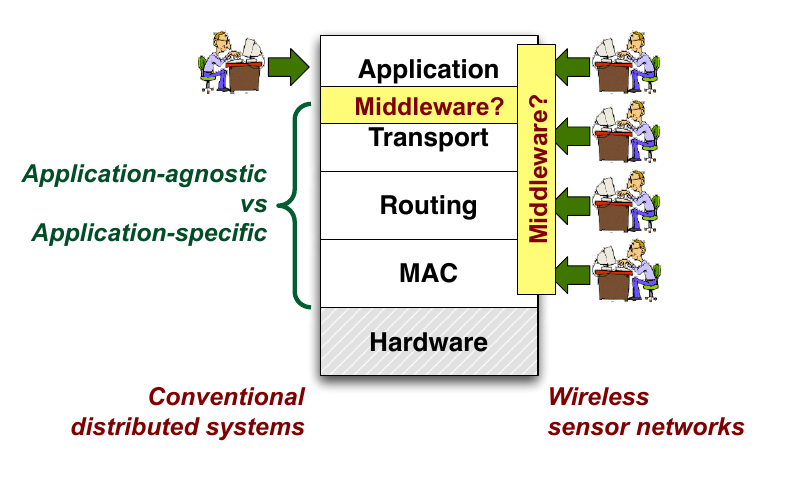
\includegraphics[width=\textwidth,keepaspectration=true]{middleware}
\end{frame}

\begin{frame}[label=sec-2-2]{Approaches to middleware}
\begin{itemize}
\item application-based; ex. Contiki, Squawk
\item component-based; ex. OpenCOM, Figaro, LooCi
\begin{itemize}
\item static
\item dynamically reconfigurable
\end{itemize}
\end{itemize}
\end{frame}

\begin{frame}[label=sec-2-3]{LooCi}
\begin{itemize}
\item Kort historisch
\item Hoe werkt t. (vb vm?)
\end{itemize}
\end{frame}
\section{Evaluating energy use}
\label{sec-3}

\begin{frame}[label=sec-3-1]{Why is it important?}
\begin{itemize}
\item WSN motes need to be long-lasting
\item energy efficiency is key
\end{itemize}
\end{frame}

\begin{frame}[label=sec-3-2]{How to measure?}
\begin{itemize}
\item oscilloscopy!
foto/filmpje
\item use triggers in software
\item derive power usage using Ohm's law
\end{itemize}
\end{frame}

\begin{frame}[label=sec-3-3]{Setup}
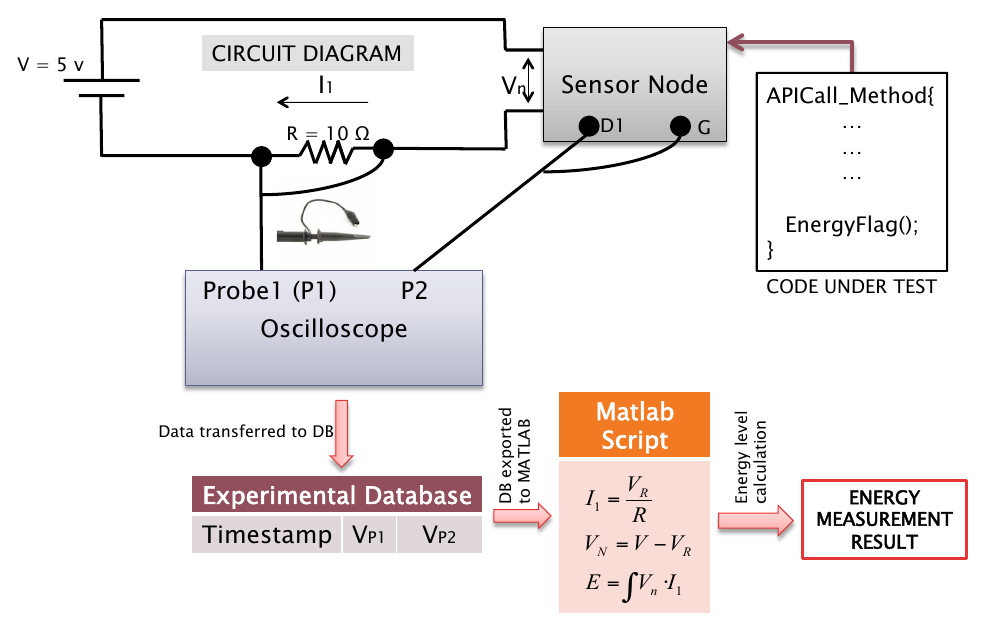
\includegraphics[width=\textwidth,keepaspectration=true]{energy_measurement_diagram}
\end{frame}

\begin{frame}[label=sec-3-4]{Plotting voltage}
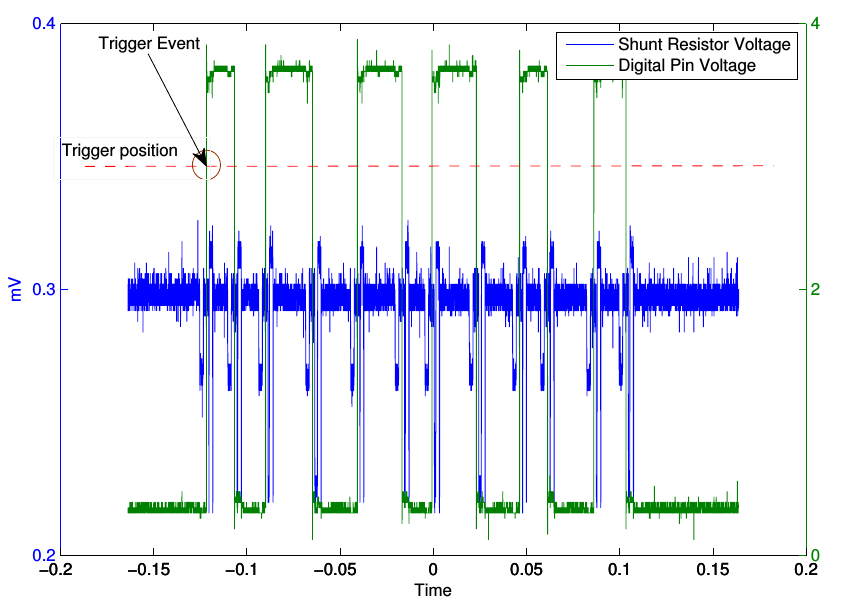
\includegraphics[width=0.95\textwidth,keepaspectration=true]{energy_measurement_plot}
\end{frame}

\begin{frame}[label=sec-3-5]{Power usage}
\begin{itemize}
\item can be derived from voltage measurements
\item can be modeled using linear regression
\end{itemize}
\end{frame}
\section{Conclusion}
\label{sec-4}
\begin{frame}[label=sec-4-1]{Where do we fit in?}
\end{frame}
\begin{frame}[label=sec-4-2]{Conclusion}
\end{frame}
\begin{frame}[label=sec-4-3]{Bibliography}
\nocite{*}
\printbibliography
\end{frame}
% Emacs 24.3.1 (Org mode N/A)
\end{document}
